\documentclass[11pt]{article}

\usepackage{hyperref}
\usepackage{graphicx}
\usepackage{todonotes}
%\usepackage{endnotes}

\usepackage{footnotebackref}



%approximately proportional to symbol
\newcommand{\approptoinn}[2]{\mathrel{\vcenter{
  \offinterlineskip\halign{\hfil$##$\cr
    #1\propto\cr\noalign{\kern2pt}#1\sim\cr\noalign{\kern-2pt}}}}}

\newcommand{\appropto}{\mathpalette\approptoinn\relax}

\title{The Demographics of Taxicab Riders}
\author{Thomas C. Proctor}
\date{\today}

%\let\footnote=\endnote

\renewcommand{\abstractname}{Executive Summary}
\newcommand{\fref}[1]{Figure~\ref{fig:#1}}
\newcommand{\prsq}{$\mbox{pseudo-}R^2$}

\begin{document}

\maketitle{}

\begin{abstract}
  In this work I create an explanatory model of the location of New York City licensed taxicab (yellow cab) drop-offs based off demographic and location data.
  These findings may help to understand the demographics of yellow cab users.
  Also, it may be combined with similar analysis of other for-hire vehicle services to compare the demographics of these services.
  This information will be especially useful to inform the re-evaluation of the regulation of for-hire vehicles which is required due to the introduction of smartphone based hailing.
  Two data sources are used: taxicab trip data provided by the NYC taxicab and livery commission and demographic data from the US Census bureau.
  As drop-offs are count data, we expect that the drop-off data is drawing from a Poisson distribution and Poisson regression is used, along with feature selection to sort through the large number of available features.
  I find that drop-offs can be well predicted by the income of census tracts, and on average, $\mbox{{\it dropoffs per-capita}}\appropto (\mbox{{\it per-capita income}})^2 $.
However, there is clearly significant influence from other factors, and the Poisson distribution based model for the randomness in taxicab drop-offs is not very accurate.
  %As explaining the number of drop-offs is a regression problem, OLS regression is chiefly used, along with feature selection to sort through the large number of available features.
  % We find that drop-offs behave dramatically differently depending on the commuting habits of residents.
  % The drop-off data in areas with very low rates of car commuting can be easily explained based only on per-capita income.
  % Meanwhile, areas with more moderate to high rates of car commuting XX.
  % These findings demonstrate that healthy public transit is critical to maintaining demand for taxi services.
  
\end{abstract}

\section{Introduction}

In 1937, in response to traffic congestion, New York City began regulating for-hire cars by limiting the total number of vehicles (yellow cabs) that can legally pick up passengers hailed from the street. This has created a system which many say is unfair to those who do not live within the core business district, as accepted wisdom says that unmet demand is high enough within the core business district that there is no incentive for drivers to leave it.
Recently, the advent of other for-hire vehicles in NYC has brought further attention to issues with yellow cabs service across geographic, income, and ethnic groups.
The city has started a system of so called ``boro cabs'', which are allowed to pick up street hails only outside of a defined central business district.
Smartphone hailing apps manage to bypass the regulation scheme based upon street hails, providing significant competition to yellow cabs, along with claims that they better serve poorer neighborhoods.
Along with the conventional wisdom about the locations where cabs can be hailed, there are also other common tropes about cab coverage, such as a bias against non-white passengers and that they are only used by the rich.

In order to answer questions about the users served by for-hire vehicles and approach questions of unmet demand, I evaluate the demographics of passengers by looking at the demographics of passenger drop-off locations. A map of this drop-off data can be seen in \fref{map}.

\begin{figure}[h]
  \centering
  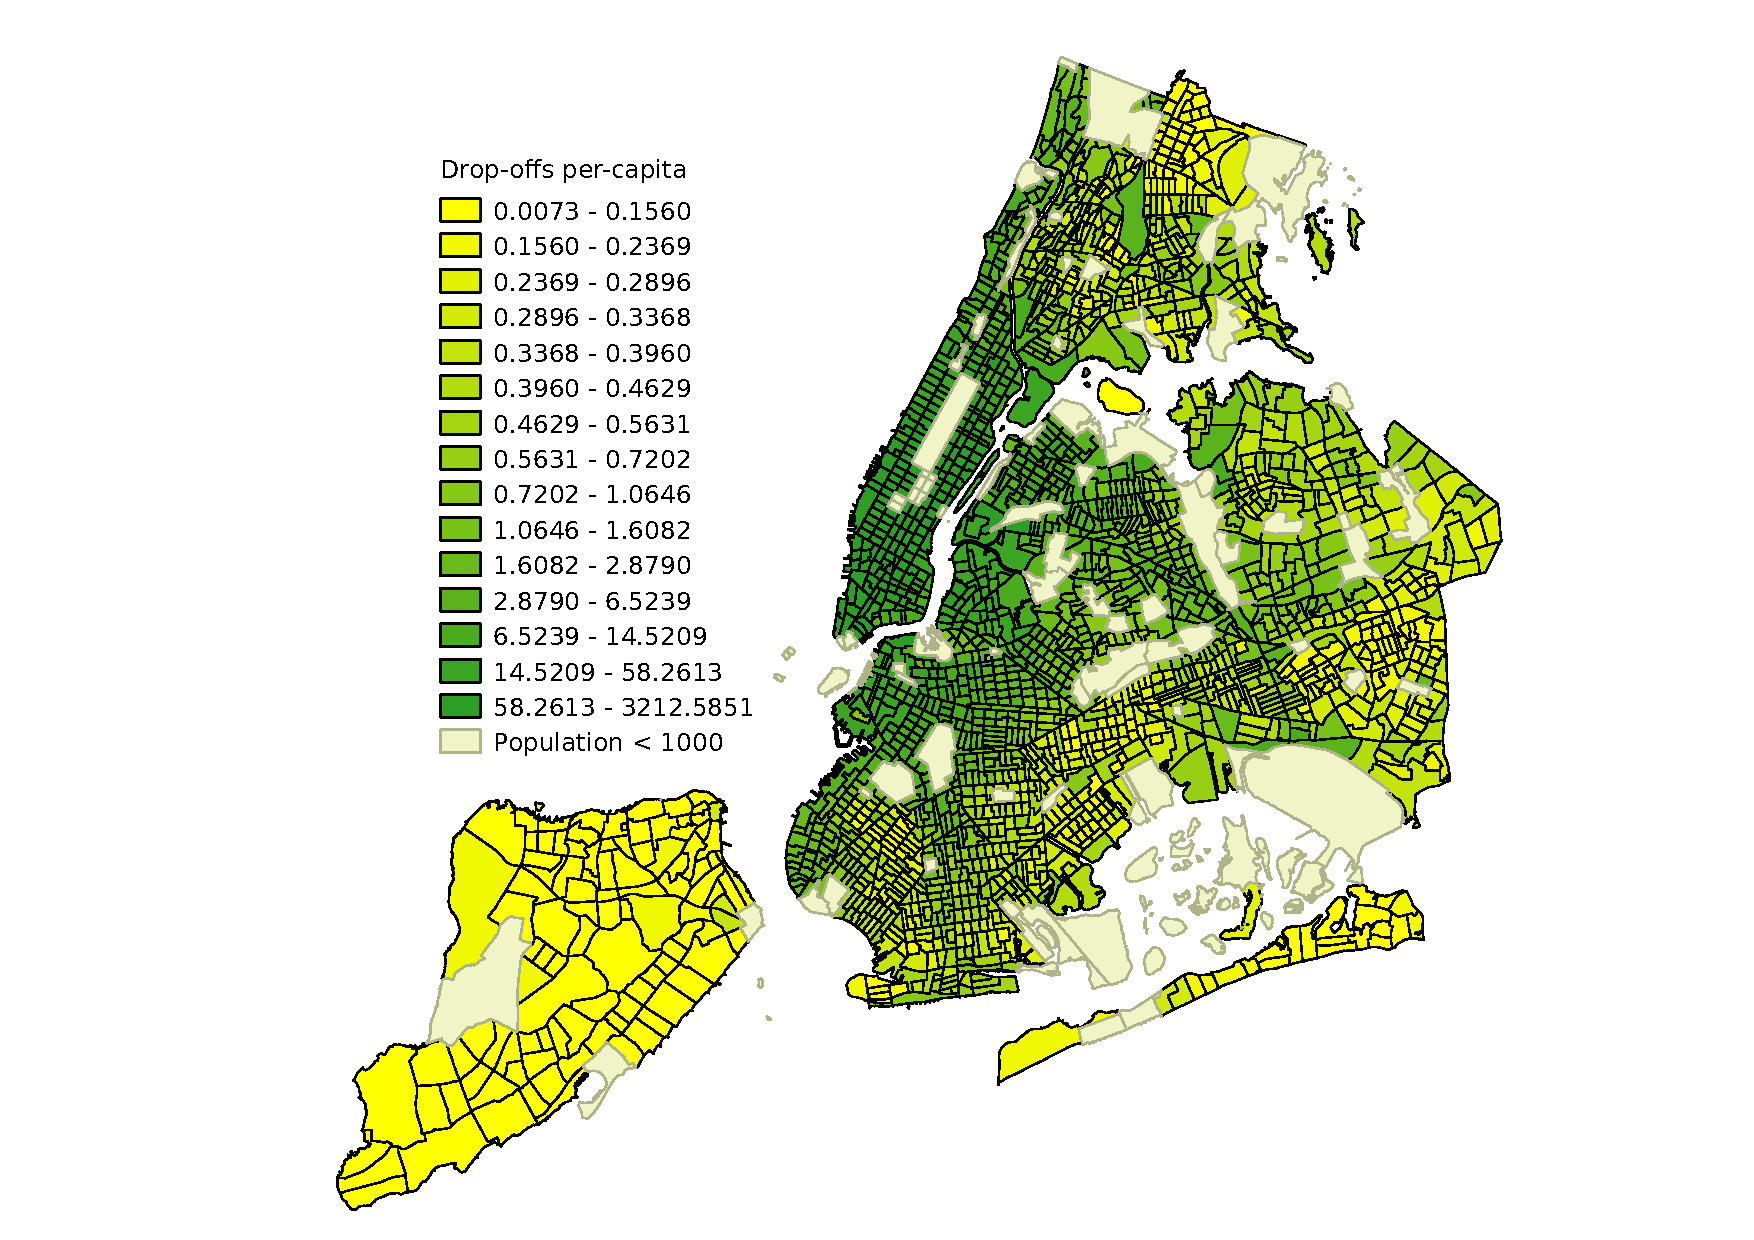
\includegraphics[width=\textwidth]{2013dropoff_map2.pdf}
  \caption{Map of New York City per-capita drop-offs. Staten Island is the island to the south-west with an overall low number of drop-offs, while Manhattan, where the chief central business district of the city is located, is the long, narrow island with a large number of drop-offs. \label{fig:map}}
\end{figure}

\subsection{Data}

I hope to be able to predict the number of drop-offs in an area based on the demographics of that area in order to understand the demographics of passengers. 
By comparing analysis for different types of for-hire vehicles, we can better understand the differences between the users of each service.

%\todo{Write out in prose}

%This is the data I have to work with:
I work with two data sources for this project.
The first is yellow cab trip data provided by the New York City Taxicab and Livery Commission\footnote{Data is available from \url{http://www.nyc.gov/html/tlc/html/about/trip_record_data.shtml} }. This data includes latitude and longitude coordinates for the start and end (pickup and drop-off) of every single yellow cab trip in NYC among lots of other trip information.
The drop-off lat. lon. coordinates are used to generate the response variable, the yearly per-capita yellow cab drop-offs in a given census tract.
%Similar data is provided by for green cabs.
When I first started exploring taxicab data, only the 2013 data had been released, so I used this data.
The second source is demographic data from the US Census Bureau\footnote{Census data is published on many websites. I've used \url{https://nhgis.org/}, as it allows you to download  only the columns you want and not waste hard drive space or time processing lots of data. The census supplies ``shapefiles" of the different geographical areas they use at \url{https://www.census.gov/geo/maps-data/data/tiger-line.html}, including tracts. The city of New York supplies shapefiles that clip to the shoreline at \url{http://www1.nyc.gov/site/planning/data-maps/open-data/districts-download-metadata.page}, as the census tracts are defined so that they include all river areas and much of the ocean. I expect that the census needs to be prepared for houseboats and changing shorelines.}.
For 2010, the full US Census is a population count that the best possible attempt to record every single resident of the US, but is mostly just counting population, with only a small amount of other information.
The American Community Survey, which runs constantly, includes many more demographic factors, including racial, income, and commute data. I used the 2009-2014 set of estimates, as the five-year estimates have reasonably low margins of error and are suggested for uses that aren't tracking demographic changes over time.
It uses sampling and gets diverse demographic information, though some of this data can have very high errors.

The data from the Census Bureau is broken up by census tract, which divides all of the United States into relatively small geographic areas which ideally are largely demographically homogeneous.
Thus, there can be a large range in total population and population density.
For example, most parks and airports in NYC have their own census tract with little to no residents.

  
% \begin{itemize}
% \item TLC data: \todo{Replace inline links with endnotes}(\url{http://www.nyc.gov/html/tlc/html/about/trip_record_data.shtml} or (just includes new data) \url{https://data.cityofnewyork.us/data?agency=Taxi+and+Limousine+Commission+\%28TLC\%29\&cat=\&type=new_view\&browseSearch=\&scope=} )
% This data includes gps coordinates for every single yellow cab trip in NYC, as well as a detailed fare breakdown, the taxi medallion, and a bunch of other info.
% The drop-off gps coordinates are used to generate our dependent variable, the yearly per-capita yellow cab drop-offs in a given census tract.
% Similar data is provided by for green cabs.

% %\item Uber FOIL data: fivethirtyeight.com did a freedom of information law request for 2014-2015 NYC Uber data, which Uber supplied, apparently quite reluctantly, as the data is not very detailed. It only contains the time and location of the pick-ups, and for 6 months, pick-up locations are organized into ``neighborhoods'', the boundaries of which are not defined. As I only have pick-ups, I will need to study pick-ups as well as drop-offs for comparison data.
% \item  Census/American Community Survey (ACS) data:
% \begin{itemize}
%         \item Income, commute data, and much, much more.
%        \item  Data from the census makes the best possible attempt to record every single resident of the US, but is mostly just counting population, with only a small amount of other info.
%         \item Data from ACS uses a random sample and gets diverse demographic information; though some of this information may have very high errors.
%         \item Available on many websites. I've used https://nhgis.org/, as it allows you to just download the columns you want and not waste hard drive space or time processing lots of data.
%         \item Unfortunately, for some fields, there is simply too much error for them to be useful. For instance, the ACS contains info on the length of time spent commuting; for car commuters, the error for their data in NYC had a median around 50\%, so it is not very useful.

%         \item The census supplies ``shapefiles" of the different geographical areas they use at \url{https://www.census.gov/geo/maps-data/data/tiger-line.html}, including tracts. The city of New York supplies shapefiles that clip to the shoreline, as the census tracts are defined so that they include all river areas and much of the ocean. I expect that the census needs to be prepared for houseboats and expanding shorelines.
%   \end{itemize}
%         %It will be interesting to see what effect race has on taxi dropoffs - does the conventional wisdom on taxis being prejudiced show up in dropoff data?
%    \item I have also taken a look at some Google maps distance data, but it wasn't very predictive on its own. Unfortunately there are limitations on how much of this data can be gathered by an individual in a day, limiting the amount of data I can gather.%Maybe combining in some of the demographic data will make it a bit more useful.


  
% \end{itemize}


\section{Methods}



%I don't have direct demographic data on the users of taxi services. 
I assume that the demographics of drop-off and pick up locations are representative of the demographics of users. As only a fraction of trips begin/end at the user's residence, this is a fairly significant assumption.
It may be possible to better control for this by finding other data sources, such as measures of the number of people working in a given area or the commercial vs. residential zoning of an area.

\subsection{Data Processing}
%\todo{Add references and hyperlinks to data processing files in endnotes}

There are over 150 million trips within NYC recorded for 2013. With the resources I have, it is not reasonable to hold all this data in RAM at once, so there is some wrangling required in order to study it.
Furthermore, finding which census tract contains the lat. lon.  point of a drop-off is a resource intensive process.
Instead of assigning census tracts point-by-point, I separate the NYC area into a fairly grid, with one one-thousandth of a degree separation between each grid line, and find the census tracts of the points in that grid\footnote{Python scripts for creating the grid to tract table and making it memory efficient can be found at my github page under \href{https://github.com/ThomasProctor/Slide-Rule-Data-Intensive/blob/master/DataStory/FinalFiles/Generate\%20gps\%20tract\%20lookup.py}{\texttt{Generate tract lookup.py}},
\href{https://github.com/ThomasProctor/Slide-Rule-Data-Intensive/blob/master/DataStory/FinalFiles/Create\%20Fipscodes\%20dictionary.py}{\texttt{Create Fipscodes dictionary.py}}, 
and \href{https://github.com/ThomasProctor/Slide-Rule-Data-Intensive/blob/master/DataStory/FinalFiles/Convert\%20gps\%20tract\%20lookup\%20low\%20memory.py}{\texttt{Convert tract lookup low memory.py}}.}.
This reduces the points needed to match to tracts to only about 24 million.
The actual work of matching the grid lat. lon.  points to tracts is done using the PostGIS add-on to PostgreSQL.
Then, lat. lon.  points can be matched to tracts by simply rounding to the nearest one-thousandth of a degree and joining the table of drop-offs with the table of grid points\footnote{A Python script for computing statistics about the drop-offs in each NYC census tract can be found at \url{https://github.com/ThomasProctor/Slide-Rule-Data-Intensive/blob/master/DataStory/FinalFiles/ComputeTractStatsFromCSV.py}.}.
Memory usage can be traded for time by only using a subset of the tracts in the table of grid points at once.
 
% First, I separate pick-up and drop-off gps data into bins by the rounded gps coordinates, and then sort this data into census tracts via PostGIS, giving a tally of the number of of trips in each census tracts.
% This automatically filters out the large number of trips that are located outside of NYC.
% While many of these are probably proper data points, many are clearly errors, probably of the GPS device.

% \begin{figure}[h]
%   \centering
%   \includegraphics[width=\linewidth]{2013dropoffs_vs_income_low_car.png}
%   \caption{ test $\mathrm{dropoffs}\approx \mathrm{income}^{2.34}/4.07\times 10^{10}$
% }

%   \label{fig:incomevdrop}
% \end{figure}

\subsection{Data Analysis}
%\todo{Add something about the census data (numbers, throwing out low pop. tracts)}
%\todo{Adding in some maps could be nice: Show the tracts you're studying, show what the boros mean, maybe try to include something showing the data studied too}



New York City contains 2168 census tracts. 
Of these, I remove 83 that have populations under 1000 persons. These tracts are mostly parks, but also include the two airports, the Brooklyn Navy Yard, and an area of Midtown Manhattan that is mainly offices and transportation hubs.
As the population of these areas is so low, we cannot expect drop-offs within them to be representative of their demographics.

Also, my analysis does not cover Staten Island, which is geographically and demographically very distinct from the rest of New York City\footnote{\url{https://en.wikipedia.org/wiki/Staten_Island}. Yes, I cited Wikipedia. The geographic position of Staten Island can be seen in \fref{map}.}.
It is the only borough with no subway connection to Manhattan, where the New York City central business district is located, so public transit connections can be much more time consuming and expensive.
Access to Manhattan by car requires crossing two bridges and driving through much of Brooklyn.
It is the only borough where non-Hispanic whites make up a majority of the population\footnote{\url{https://en.wikipedia.org/wiki/Demographics_of_Manhattan}}, and its car ownership rate by household of 84\% dwarfs that of the next closest, Queens, with 64\%\footnote{\url{http://www.nycedc.com/blog-entry/new-yorkers-and-cars}}.
Unlike most of New York City, it is almost entirely suburban, and the separation between Staten Island is so pronounced that a referendum passed in 1993 to secede from the city, though the state prevented its implementation.

\todo{Clean up feature selection notebook, add github link to endnotes}
Feature selection of a large body of demographic data, including commute patters, racial make-up, and economic data of residents indicates that per-capita income is the most promising predictor for drop-offs in a given census tract. 
This is not surprising. Taxicabs are a luxury service. In NYC, taxi cabs compete with public transit that costs about as much per trip as the minimum charge for a taxi, and just a little bit over 1\% of New York commuters commute mainly via taxicab. 
Thus, I would expect that those with more income are more likely to take cabs, and this is the case. 
%\todo{Write about removing Staten Island}

\subsubsection{Poisson Regression}



The log-log plot  of per-capita drop-offs vs per-capita income shown in \fref{dropoffsvsincome} indicates a roughly linear relationship of the logarithms of the two variables. The deviance from this linear behavior in the lower left of this plot can be explained by the fact that the data is drawn from a Poisson distribution, and data will not be symmetrically distributed around the mean.
%The logarithmic behavior of the drop-offs is common for Poisson distributed data. 
\begin{figure}[h]
  \centering
  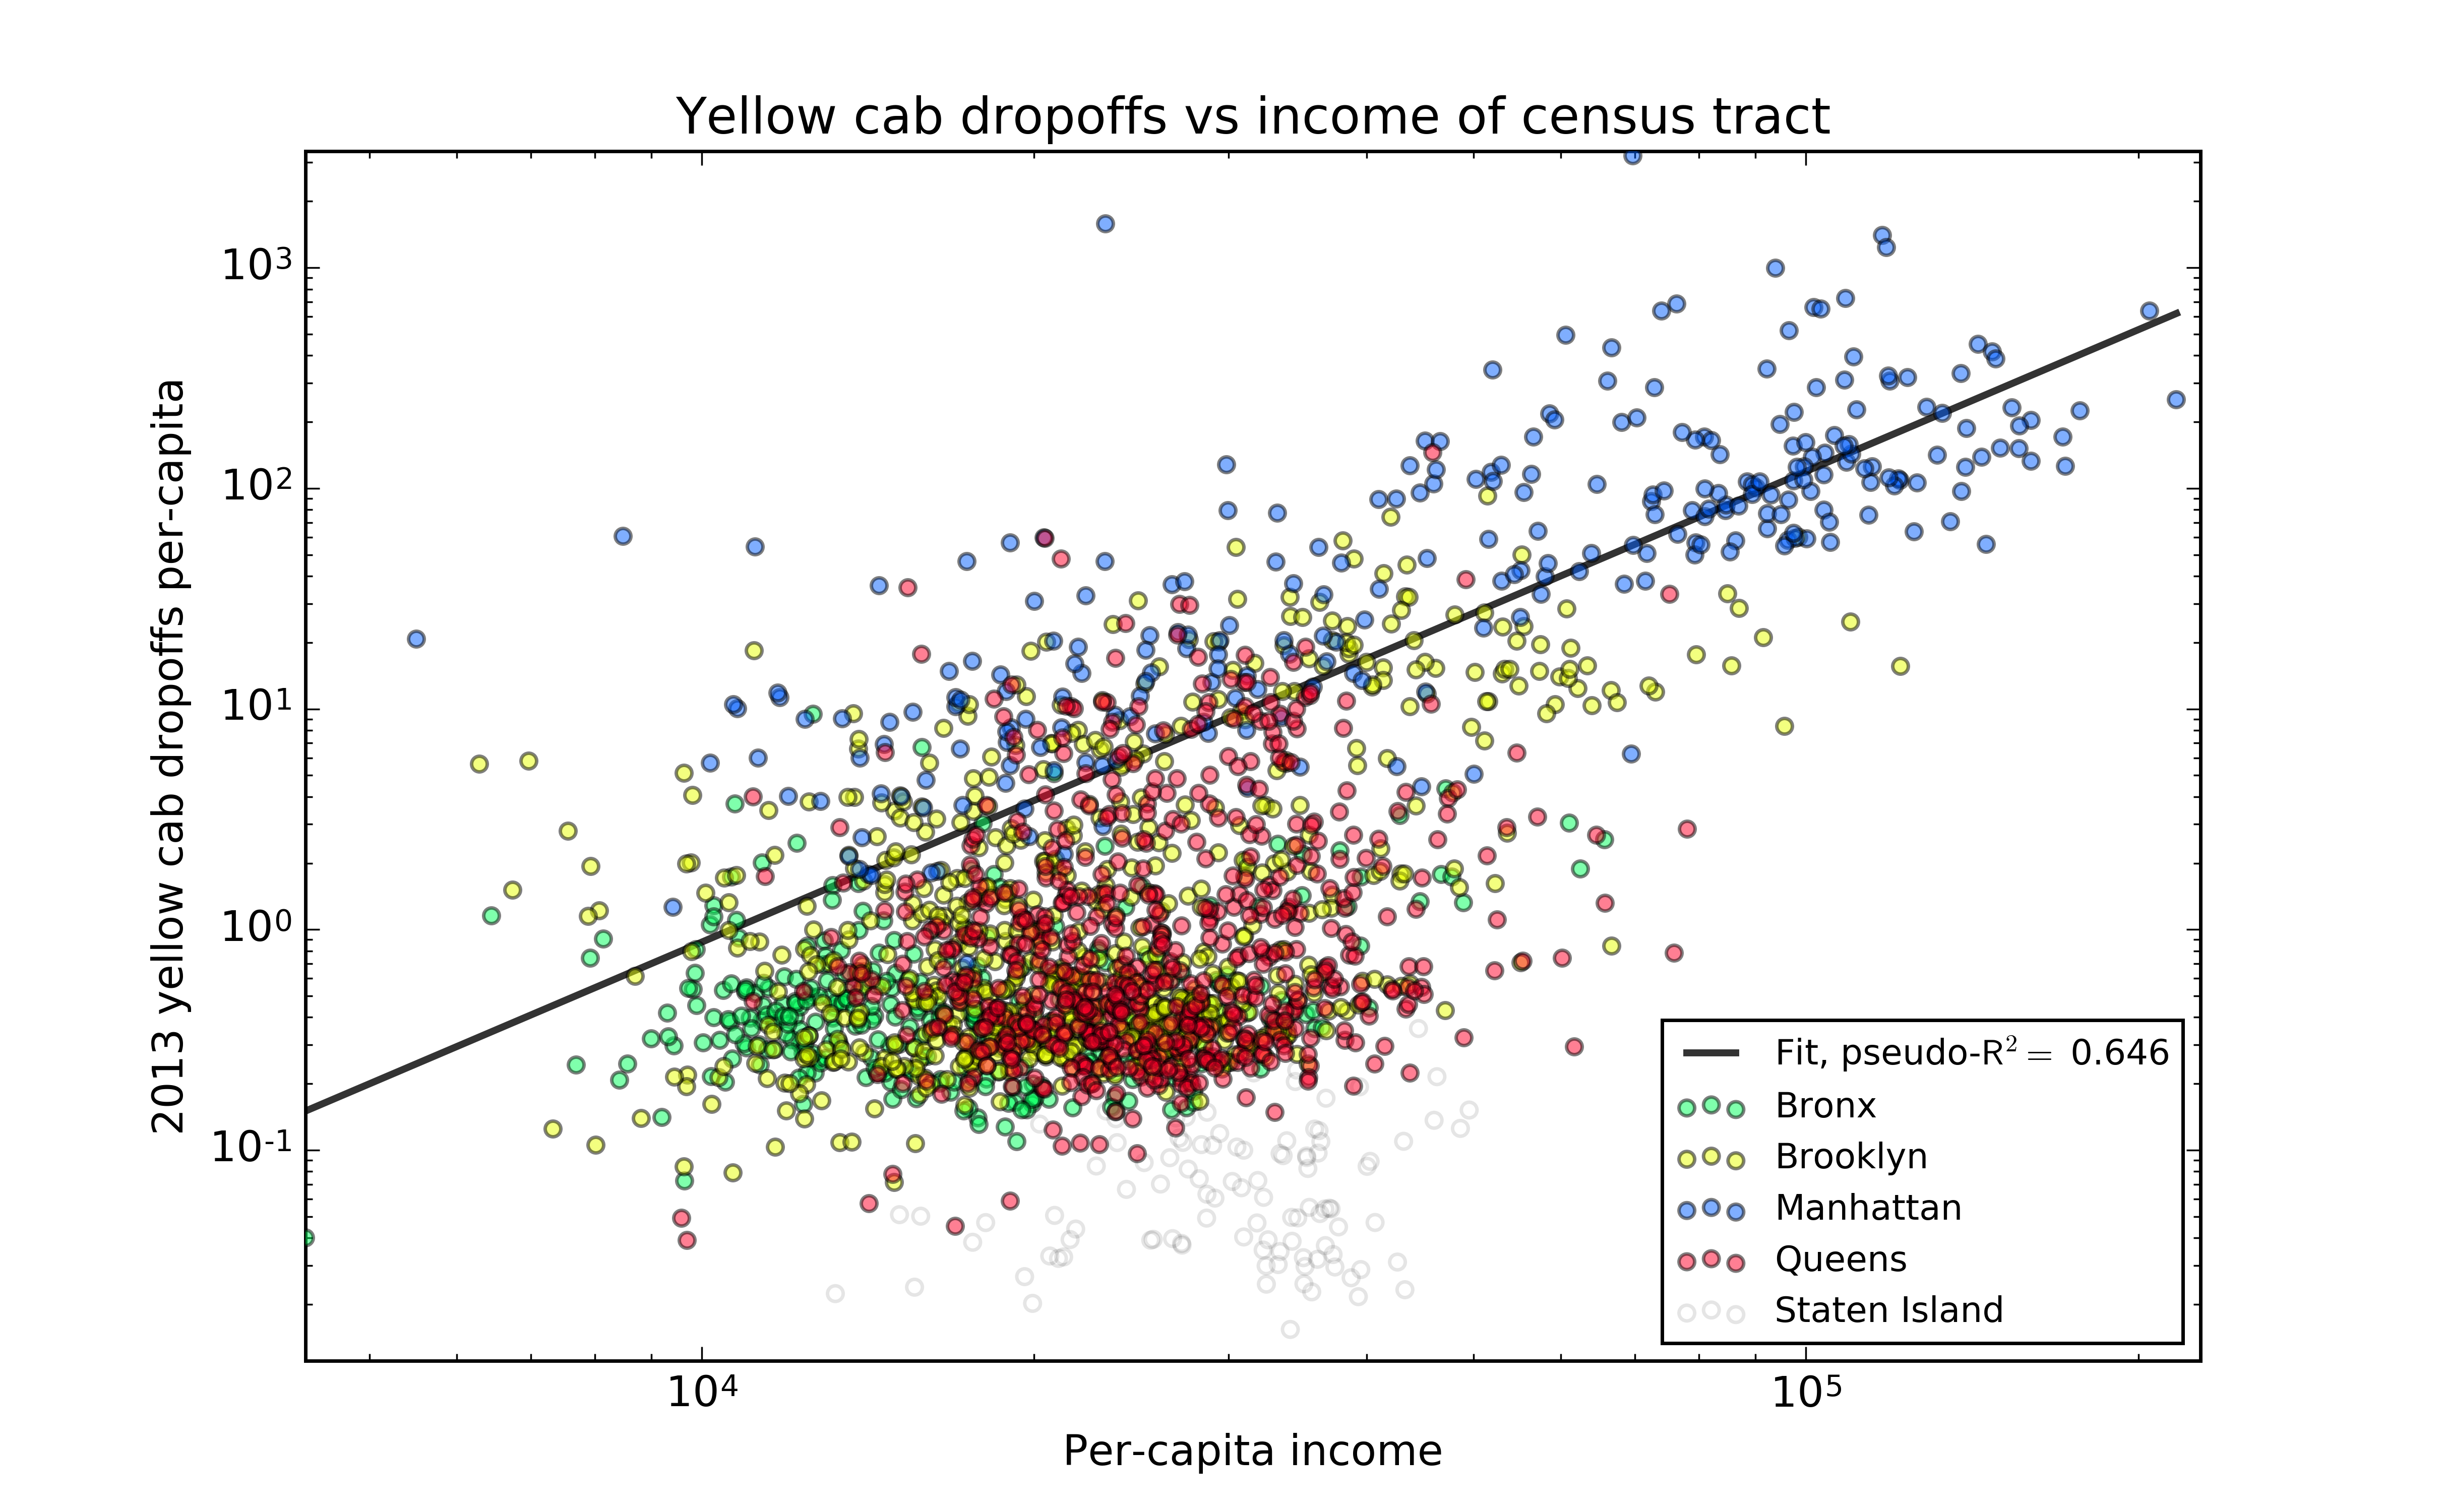
\includegraphics[width=\textwidth]{2013count_dropoffs_vs_income_low_car_poisson.png}
  \caption{Per-capita drop-offs vs per-capita income with a Poisson model. The fit is given in equation \ref{eq:PoissonFit}.\label{fig:dropoffsvsincome}}
\end{figure}
Using
\begin{equation}
  \log d - \log p = \theta_c + \theta_j \log j
\end{equation}
as my model, where $d$ is the drop-offs in a given census tract, $p$ is the population (included in the model as an offset), and $\theta_c$ and $\theta_j$ are unknown parameters of the model.
I do a Poisson regression on this data and find that 
\begin{equation}
  \label{eq:PoissonFit}
  y\approx \frac{j^2}{4.7\times 10^8},
\end{equation}
where $y$ is the drop-offs per-capita in a given census tract, and $j$ is the per-capita income of that tract\footnote{The code for performing the Poisson regression analysis can be found on my github under \href{https://github.com/ThomasProctor/Slide-Rule-Data-Intensive/blob/master/DataStory/FinalFiles/Poisson_regression.ipynb}{\texttt{Poisson\_regression.ipynb}}. This jupyter notebook also contains all the code to generate the associated figures and other analysis.}.
This fit is illustrated in \fref{dropoffsvsincome}.
%\todo{Clean up Poisson analysis notebook and add footnote}





% Using the deviance residuals of our quasi-Poisson regression, defined as

% \begin{equation}
% r^D\equiv \frac{\mathrm{sign}( y_i - \hat{y}_i)}{\tau} \sqrt{y_i \log\left(\frac{y_i}{\hat{y}_i}\right) -(y_i-\hat{y}_i)},
% \end{equation}
% where $y_i$ is the $i^{\mathrm{th}}$ drop-off data point,  $\hat{y}_i$ is the corresponding prediction, and $\tau$ is the dispersion parameter, the factor that relates the quasi-Poisson model variance to that of an ordinary Poisson model.
% For our data, $\tau=85735$
One of the more useful methods for judging the quality of Poisson regression is by looking at the deviance, which is the factor that is minimized in the regression algorithm.
I find a very high deviance of $2\times 10^8$, which gives a p-value of 1 when compared as a hypothesis with the saturated model as the null hypothesis.
This isn't all that surprising.
A Poisson distribution has a variance equal to it's mean.
Because there are obviously more factors at play than the predictors that we have used, we would expect that there will be a lot of extra variance than that expected by the pure Poisson distribution. This {\it overdispersion} is generally the rule rather than the exception with real world data.

The normal way to account for this overdispersion is by relaxing the requirement that the variance is equal to the mean, and instead have the variance equal to $\tau \lambda$, where $\lambda$ is the mean, a function of the predictors, and $\tau$ is a fitted constant called the {\it dispersion parameter}. The resulting model, called a {\it quasi-Poisson} model, will always have the exact same prediction for the mean as the corresponding Poisson model, as the only thing that has changed is the random part of the model.

Using a quasi-Poisson model, the deviance is lowered significantly to 386, and the p-value is reduced to zero.
However, this should be taken with a grain of salt, as the dispersion parameter is an incredibly high $5\times10^5$, indicating that there is a huge amount of extra variance above and beyond the Poisson model expectation.

The quality of the random component of the model can also be judged by looking at the {\it Anscombe residuals}, which transform the residuals so that they should have an approximately normal distribution if the model is correct.
However, the quantile-quantile plot shown in \fref{qqplot} shows that distribution of the Anscombe residuals is far from normal.
The distribution is narrow around the mean, with relatively longer tails than that of a normal distribution.

\begin{figure}[h]
  \centering
  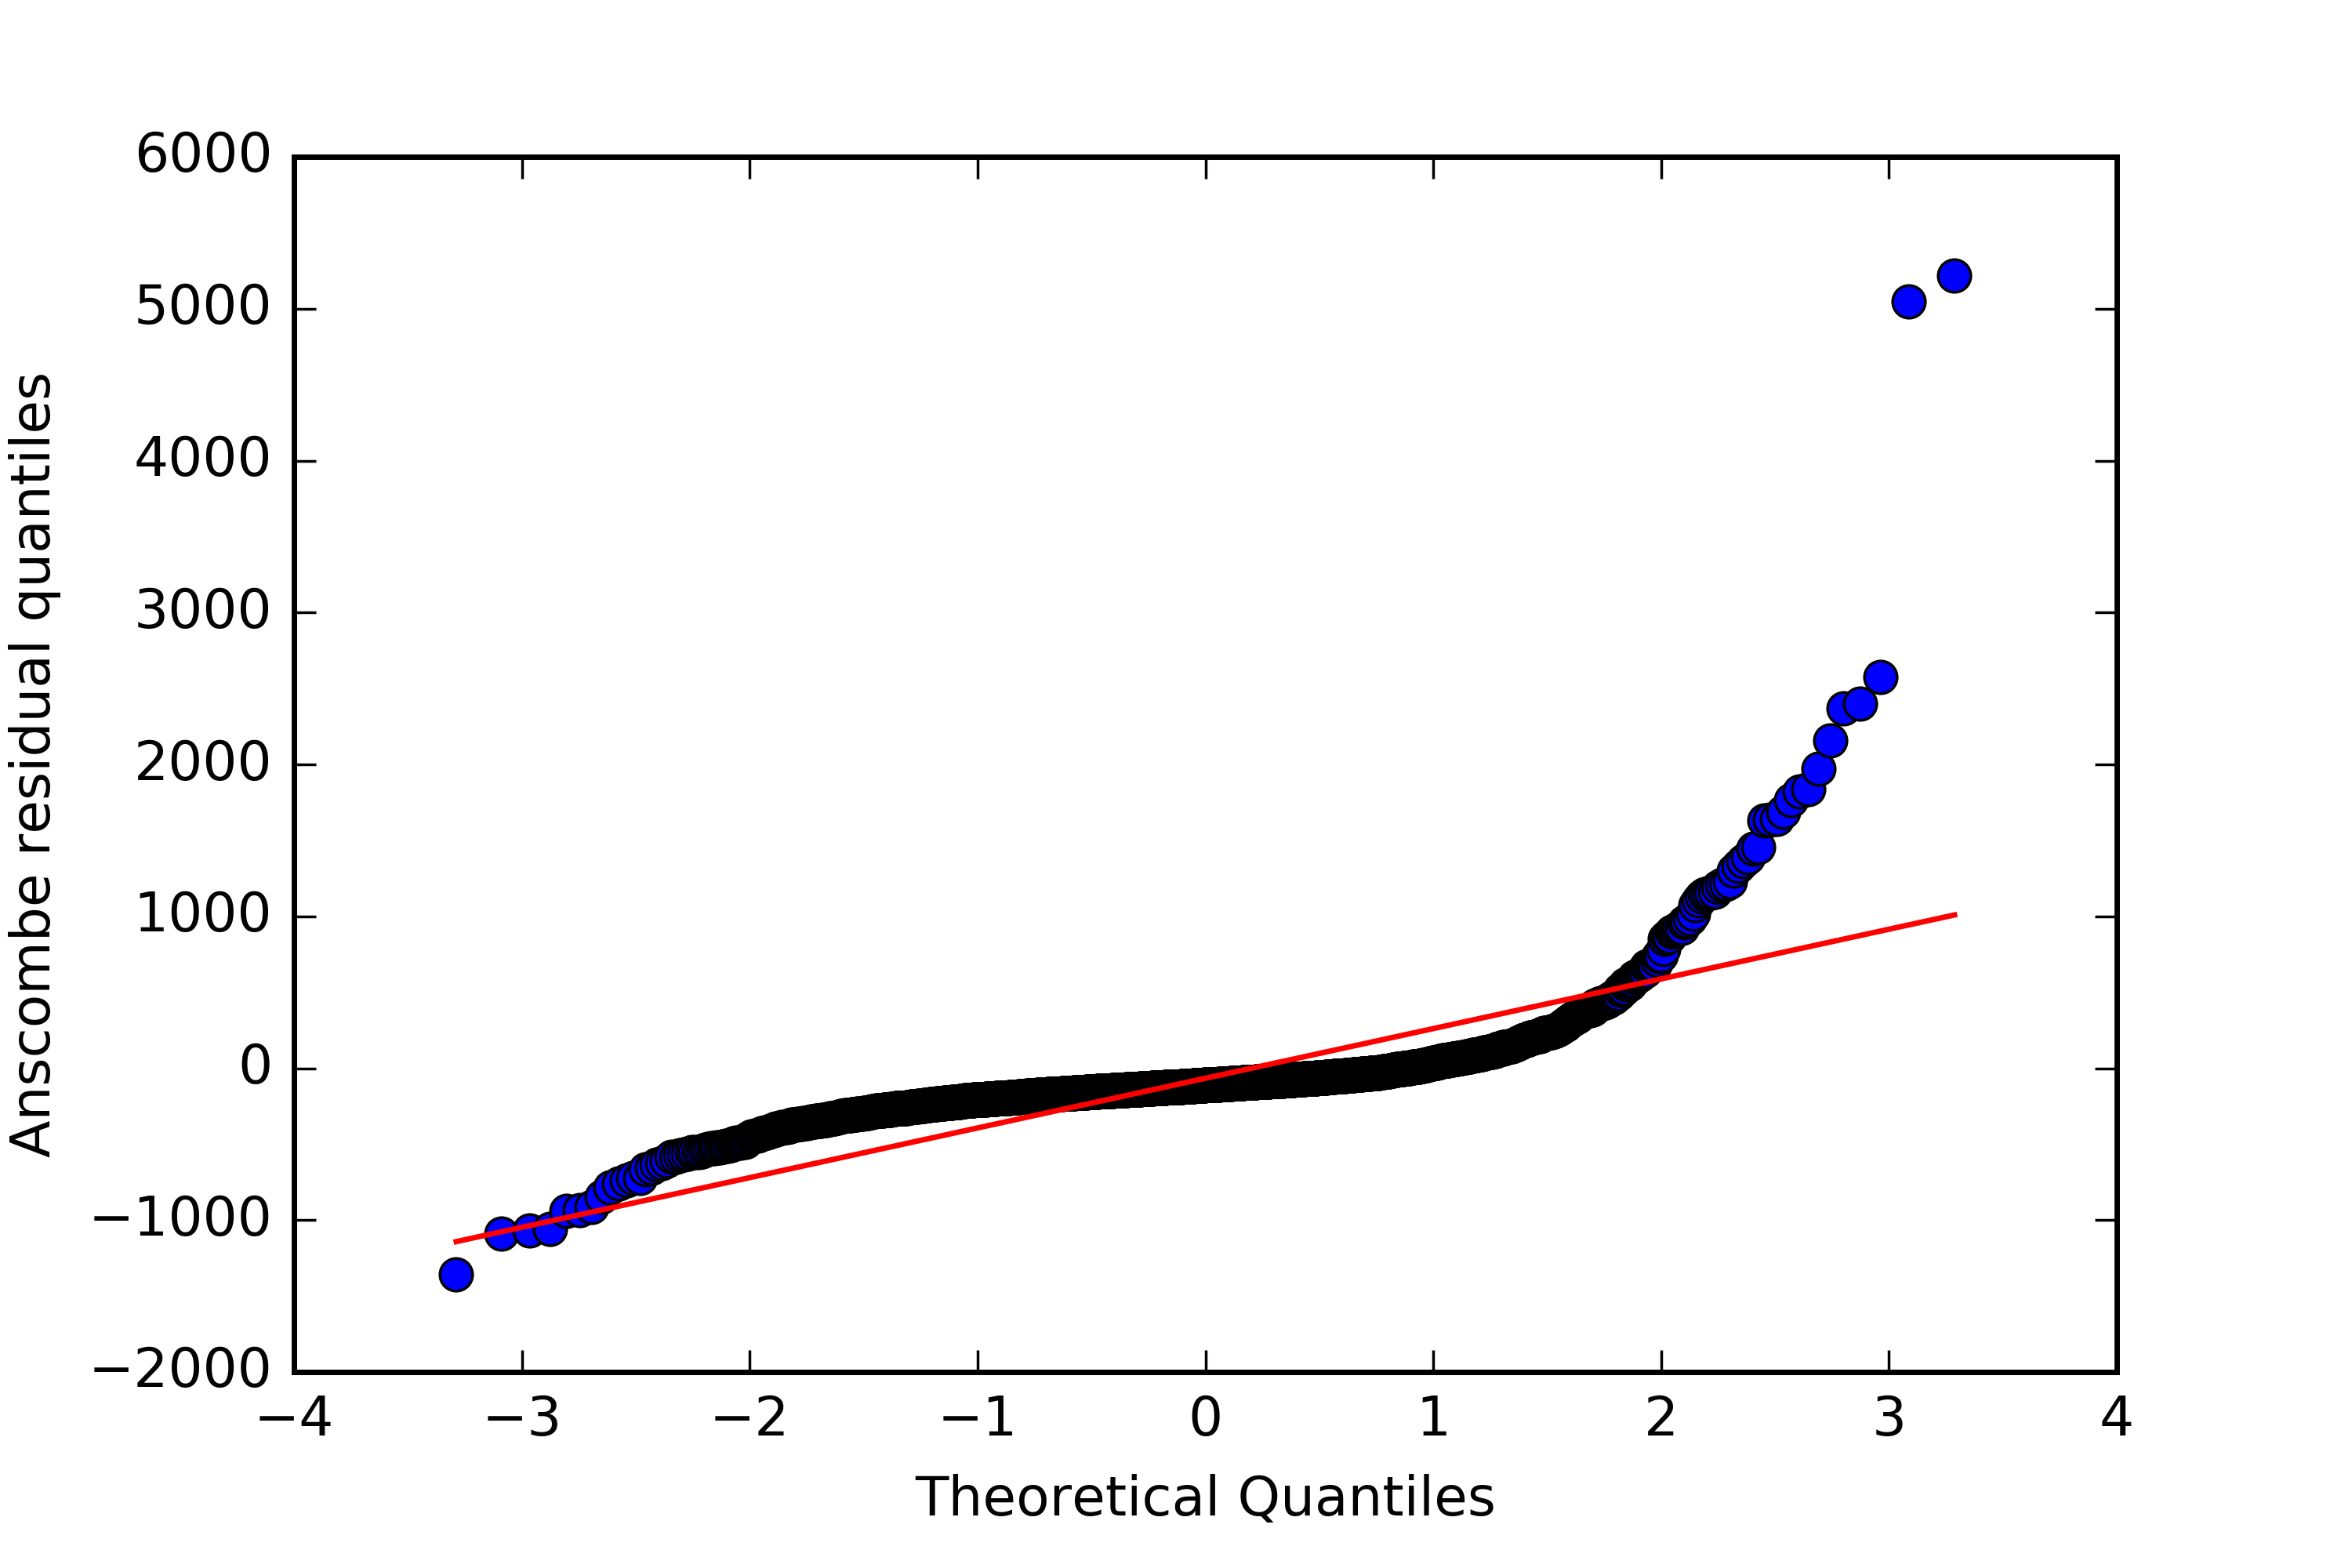
\includegraphics[width=\textwidth]{2013quasi-poisson_QQ.png}
  %\includegraphics[width=\halflength]{2013_poisson_QQ_line.png}
  \caption{ Q-Q plot for a quasi-Poisson fit. If the residuals followed a normal distribution, they would lie on the red line.
  \label{fig:qqplot}}

\end{figure}

Using the dispersion, we can find a parameter analogous to the $R^2$ used in ordinary least squares which measures the improvement over the null model, called {\it Mcfadden's $\mbox{pseudo-}R^2$}. This \prsq \ is 0.65 for our quasi-Poisson model, indicating that a dramatic improvement over the null model, although the behavior of the residuals runs counter to the expectations of the model, as indicated by both the very high value for $\tau$ and the poor fit to a normal distribution.

%\todo{Write up summary of Poisson distribution data analysis}
%\todo{Maybe clear up document about the details of the Poisson analysis and publish it separately}
%\todo{Include q-q plot}
%\todo{get rid of q-q plot title}
%\todo{change color scheme of data plot}


\section{Conclusions}

Based on this analysis, we can see that per-capita income is an impressive predictor for taxicab drop-offs, with a \prsq of 0.65.
However, the high dispersion parameter, along with the poor fit of the deviance residuals to a normal distribution indicates that the model may still have much room for improvement.
A possible avenue may be adding more demographic predictors, such as the average commute time, car usage, spatial position, or the racial make-up of census tracts. Borough, which may be a rough proxy for any of these possible predictors can be seen to correlate will with drop-offs in \fref{dropoffsvsincome}.
However, while there may be interesting information to be gleaned from exploring which predictors are the most successful, the room for improvement in this model largely lies in the distribution of the predicted error, and thus would probably be relatively marginal.

It is also possible that no improvement can be achieved from a demographic data based approach.
It may be that the effect from factors like transit hubs and cultural institutions that are particular to each individual census tract cannot be fully expressed through demographic data, and may not be able to be reasonably tracked by any data.

I, for one, find the simplicity of this model appealing: per-capita dropoffs are proportional to the square of per-capita income.
While there are clearly more details, the simple take away here is very satisfying.

\todo{Write a lay-person readable blog post.}

%\todo{Write conclusion}
%\todo{Talk about boro as a possible predictor, but also mention others}



% - mostly. People with more income are also more likely to own a car themselves, and thus not need a taxicab in the first place. 
%Thus, if we look at just the census tracts where very few people commute by car, we find a nice, simple relationship between per-capita taxicab drop-offs (dropoffs) and per-capita income (income):
% $$
% \mathrm{dropoffs}\approx \frac{\mathrm{income}^{2.34}}{4.07\times 10^{10}}
% $$
% After discarding 10 high leverage points and outliers, this data set is pretty close to perfect for regression, with a fairly normal distribution of the data.
% The outliers consist of three major transportation hubs and two census tracts whose only residences are probably homeless shelters or college dorms, and are not surprising as outliers. The high-leverage (i.e. extreme income) points are all tracts on the Upper East Side next to central park, which I believe may be the highest income tracts in the nation.
% This fit is fairly strong, and with $R^2=0.71$, much of the variance is explained through regression.

% This data, however, only includes 672 of the 2083 census tracts with populations above 1000 (tracts with lower populations are largely parks and airports; there is no reason to think that taxicab drop-offs in these locations are representative of residents).
% The other 1411 data points with rates of car commuting above 20\% don't show a correlation with income, and it seems like they may be best explained with data that combines public transit usage with some measure of travel times to the central business district, though I am still working on finding the best data and the best way to combine them.




%\theendnotes



\newpage


\listoftodos
\end{document}
